%!TEX program = xelatex

\documentclass[a4paper, openany, oneside]{memoir}
\usepackage[no-math]{fontspec}
\usepackage{pgfplots}
\usepackage{float}
\pgfplotsset{compat=newest}
\usepackage{commath}
\usepackage{mathtools}
\usepackage{amssymb}
\usepackage{amsthm}
\usepackage{booktabs}
\usepackage{todonotes}
\usepackage{mathtools}
\usepackage{xcolor}
\usepackage[separate-uncertainty=true, per-mode=symbol]{siunitx}
\usepackage{listings}
\usepackage[american inductor, european resistor]{circuitikz}
\usepackage{amsmath}
\usepackage{amsfonts}
\usepackage{ifxetex}
\usepackage[dutch,english]{babel}
\usepackage[backend=bibtexu,texencoding=utf8,bibencoding=utf8,style=ieee,sortlocale=en_GB,language=auto]{biblatex}
\usepackage[strict,autostyle]{csquotes}
\usepackage{import}
\usepackage{standalone}
\usepackage{bookmark,hyperref}
\usepackage{xcolor,mdframed}
\usepackage{tikz}
\usepackage{framed}
\usepackage{float}
\usepackage{tabularx}
\usepackage{graphicx,adjustbox}
\usepackage{rotating}
\usepackage{pdfpages}
\usepackage{enumitem}
\usepackage{calc}
\usepackage{pgfplots}
\usepackage{filecontents}
\usepackage{caption}
\usepackage{subcaption}
\usepackage{lettrine}

\newcolumntype{Y}{>{\raggedright\arraybackslash}X} % Left-justified text in tabularx environment

\ifxetex{} % Fonts laden in het geval dat je met Xetex compiled
    \usepackage{fontspec}
    \defaultfontfeatures{Scale=MatchLowercase, Ligatures=TeX} % To support LaTeX quoting style
    %\setromanfont{Palatino Linotype} % Tover ergens in Font mapje in root.
    \setsansfont{Avenir Next LT Pro}
    \setromanfont{Adobe Caslon Pro} % Tover ergens in Font mapje in root.
    \setmonofont{Source Code Pro}
\else % Terug val in standaard pdflatex tool chain. Geen ondersteuning voor OTT fonts
    \usepackage[T1]{fontenc}
    \usepackage[utf8]{inputenc}
\fi
\usepackage[noabbrev, capitalize]{cleveref}
\usepackage{ifthen}
\usepackage{titlesec}
\usepackage{titlecaps}

\newcommand{\references}[1]{\begin{flushright}{#1}\end{flushright}}
\renewcommand{\vec}[1]{\boldsymbol{\mathbf{#1}}}
\newcommand{\uvec}[1]{\boldsymbol{\hat{\vec{#1}}}}
\newcommand{\mat}[1]{\boldsymbol{\mathbf{#1}}}
\newcommand{\fasor}[1]{\boldsymbol{\tilde{\vec{#1}}}}
\newcommand{\cmplx}[0]{\mathrm{j}}
\renewcommand{\Re}[0]{\operatorname{Re}}
\newcommand{\Cov}{\operatorname{Cov}}
\newcommand{\Var}{\operatorname{Var}}
\newcommand{\proj}{\operatorname{proj}}
\newcommand{\Perp}{\operatorname{perp}}
\newcommand{\col}{\operatorname{col}}
\newcommand{\rect}{\operatorname{rect}}
\newcommand{\sinc}{\operatorname{sinc}}
\newcommand{\lcm}{\operatorname{lcm}}
%\newcommand{\gcd}{\operatorname{gcd}}
\newcommand{\F}{\mathcal{F}}
\newcommand{\DTFT}{\mathcal{F}_*}
\newcommand{\conj}[1]{#1^*}
\renewcommand{\mod}{\operatorname{mod}}
\newcommand{\rot}{\operatorname{rot}}
\newcommand{\vecsc}[1]{\vec{\textsc{\textbf{#1}}}}
\renewcommand{\ss}[1]{_{#1}}

% Label without linebreak breaker
\newcommand{\lab}[1]{\label{#1}\nolinebreak}

\newtheorem{definition}{Definition}
\newtheorem{theorem}{Theorem}


\DeclareSIUnit{\voltampere}{VA} %apparent power
\DeclareSIUnit{\pii}{\ensuremath{\pi}}

\hypersetup{%setup hyperlinks
    colorlinks,
    citecolor=black,
    filecolor=black,
    linkcolor=black,
    urlcolor=black
}

% Example boxes
\usepackage{fancybox}
\usepackage{framed}
\usepackage{adjustbox}
\newenvironment{simpages}%
{\AtBeginEnvironment{itemize}{\parskip=0pt\parsep=0pt\partopsep=0pt}
\def\FrameCommand{\fboxsep=.5\FrameSep\shadowbox}\MakeFramed{\FrameRestore}}%
{\endMakeFramed}

% Impulse train
\DeclareFontFamily{U}{wncy}{}
\DeclareFontShape{U}{wncy}{m}{n}{<->wncyr10}{}
\DeclareSymbolFont{mcy}{U}{wncy}{m}{n}
\DeclareMathSymbol{\Sha}{\mathord}{mcy}{"58}

\setlength{\parindent}{0pt}
\nonzeroparskip

% Block environment configuration
\newcommand{\BlockLeftMargin}{20pt}
\newcommand{\BlockLeftMarginText}{25pt}
\newcommand{\BlockLeftMarginTextSpacing}{10pt}

% Own colours
\definecolor{gray75}{gray}{0.75}

% Block environment
\newenvironment{block}[3]{%
\makebox{\hspace{-\spinemargin}%
\begin{tikzpicture}[overlay]
    \draw [thick,color=gray75] (\BlockLeftMargin, 0) -- (\paperwidth - \spinemargin, 0);
    \node at (\BlockLeftMarginText, -0.9) [align=left, text width=\spinemargin - \BlockLeftMarginText - \BlockLeftMarginTextSpacing, anchor=west, text depth=1cm] {\textbf{\textsc{#1}}\newline\textit{#3}};
\end{tikzpicture}}%
\nopagebreak\\[0.25em]\ifthenelse{\equal{#2}{}}{}{(\textit{#2}.) }\nopagebreak\nolinebreak}
{\nopagebreak\\[-0.25em]%
\makebox{\hspace{-\spinemargin}%
\begin{tikzpicture}[overlay, remember picture]
    \draw [thick,color=gray75] (\spinemargin,0) -- (\paperwidth - \spinemargin,0);
\end{tikzpicture}} \vspace{0.5em}}

% Theorem
\newcounter{blockTheoremCounter}
\crefname{blockTheoremCounter}{Theorem}{Theorems}
\Crefname{blockTheoremCounter}{Theorem}{Theorems}

\newenvironment{blockTheorem}[1][]{%
\refstepcounter{blockTheoremCounter}%
\begin{block}{theorem \theblockTheoremCounter}{#1}{}}
{\end{block}}

% Definition
\newcounter{blockDefinitionCounter}
\crefname{blockDefinitionCounter}{Definition}{Definitions}
\Crefname{blockDefinitionCounter}{Definition}{Definitions}

\newenvironment{blockDefinition}[1][]{%
\refstepcounter{blockDefinitionCounter}%
\begin{block}{definition \theblockDefinitionCounter}{#1}{}}
{\end{block}}

% Proof
\newcounter{blockProofTheoremCounter}
\crefname{blockProofTheoremCounter}{Proof}{Proofs}
\Crefname{blockProofTheoremCounter}{Proof}{Proofs}

\newenvironment{blockProofTheorem}[1]{%
\refstepcounter{blockProofTheoremCounter}%
\begin{block}{proof of \\ theorem #1}{}{}}
{\qed\end{block}}

% Detail
\newcounter{blockDetailCounter}
\crefname{blockDetailCounter}{Detail}{Details}
\Crefname{blockDetailCounter}{Detail}{Details}

\newenvironment{blockDetail}[1][]{%
\refstepcounter{blockDetailCounter}%
\begin{block}{detail \theblockDetailCounter}{#1}{}}
{\end{block}}

% Redesign chapter headings
\newcommand{\chapternumber}{\thechapter}
\newcommand{\hsp}{\hspace{20pt}}
\titleformat{\chapter}[hang]{\Huge\bfseries}{\chapternumber\hsp\textcolor{gray75}{|}\hsp}{0pt}{\Huge\bfseries}

% Remove headers
% \addtopsmarks{headings}{}{
%   \createmark{chapter}{left}{nonumber}{}{}
% }
% \pagestyle{headings} % Activate changes

% Capitalise headers in a regular way
\renewcommand*{\memUChead}[1]{\titlecap{#1}}

% \hfill for math mode
\newcommand{\pushright}[1]{\intertext{\hfill$\displaystyle #1$}}
\newcommand{\pushline}{\hskip \textwidth minus \textwidth}
\newcommand{\matlab}{\textsc{Matlab}}

\definecolor{code-grey}{HTML}{DDDDDD}
\newcommand{\lib}[1]{\textsf{#1}}
\newcommand{\file}[1]{\textsf{#1}}
\newcommand{\func}[1]{\colorbox{code-grey}{\texttt{#1}}}
\newcommand{\class}[1]{\colorbox{code-grey}{\texttt{#1}}}

% Setup actiepunten
\newenvironment{important}[1][]{%
   \begin{mdframed}[%
      backgroundcolor={red!15}, hidealllines=true,
      skipabove=0.7\baselineskip, skipbelow=0.7\baselineskip,
      splitbottomskip=2pt, splittopskip=4pt, #1]%
   \makebox[0pt]{% ignore the withd of !
      \smash{% ignor the height of !
         \fontsize{32pt}{32pt}\selectfont% make the ! bigger
         \hspace*{-19pt}% move ! to the left
         \raisebox{-2pt}{% move ! up a little
            {\color{red!70!black}\sffamily\bfseries !}% type the bold red !
         }%
      }%
   }%
}{\end{mdframed}}
\newcommand{\excl}[1]{
\begin{important}
  \textbf{#1}
\end{important}
}

\makeatletter
\newcommand\footnoteref[1]{\protected@xdef\@thefnmark{\ref{#1}}\@footnotemark}
\makeatother

% Allow page breaks in display environments
%\allowdisplaybreaks
% S unit for use in Mega Samples per second
\DeclareSIUnit\sample{S}

\newcommand{\CC}{C\nolinebreak\hspace{-.05em}\raisebox{.3ex}{ \textbf{+}}\nolinebreak\hspace{-.10em}\raisebox{.3ex}{\textbf{+}}}
\def\CC{{C\nolinebreak[4]\hspace{-.05em}\raisebox{.3ex}{\textbf{++}}}}


\newcommand{\partauthor}[1]{\gdef\@partauthor{#1}}
\renewcommand{\printparttitle}[1]{
  \parttitlefont #1\\
  \vspace{1.5cm}
  \textnormal{\Large \@partauthor}
}
\addbibresource{../../../includes/bibliography.bib}

\title{Compressive Sensing - An Overview}

\author{W.P. Bruinsma \and R.P. Hes \and H.J.C. Kroep \and T.C. Leliveld \and W.M. Melching \and T.A. aan de Wiel}

\raggedbottom

\begin{document}
\chapter{Model - Cogradio}
\label{cha:model}
In this chapter we will discuss the model part of our system. All the software discussed in this chapter is contained in \lib{cogradio} in the source. We will describe each step of the process from sampling to detection. For each step we will describe which methods we used and what choices we made.

\section{Source}
\label{sec:source}
All our sources are derived from one base source, that defines the methods that every source should implement: the constructor and a \func{generate} function. This generate function should return the requested number of samples from a specific source. The rest of our source can be divided in two categories, the simulated sources used for testing our algorithms and real-world sources that connect to the USRPs to retrieve samples.

\begin{figure}
    \centering
    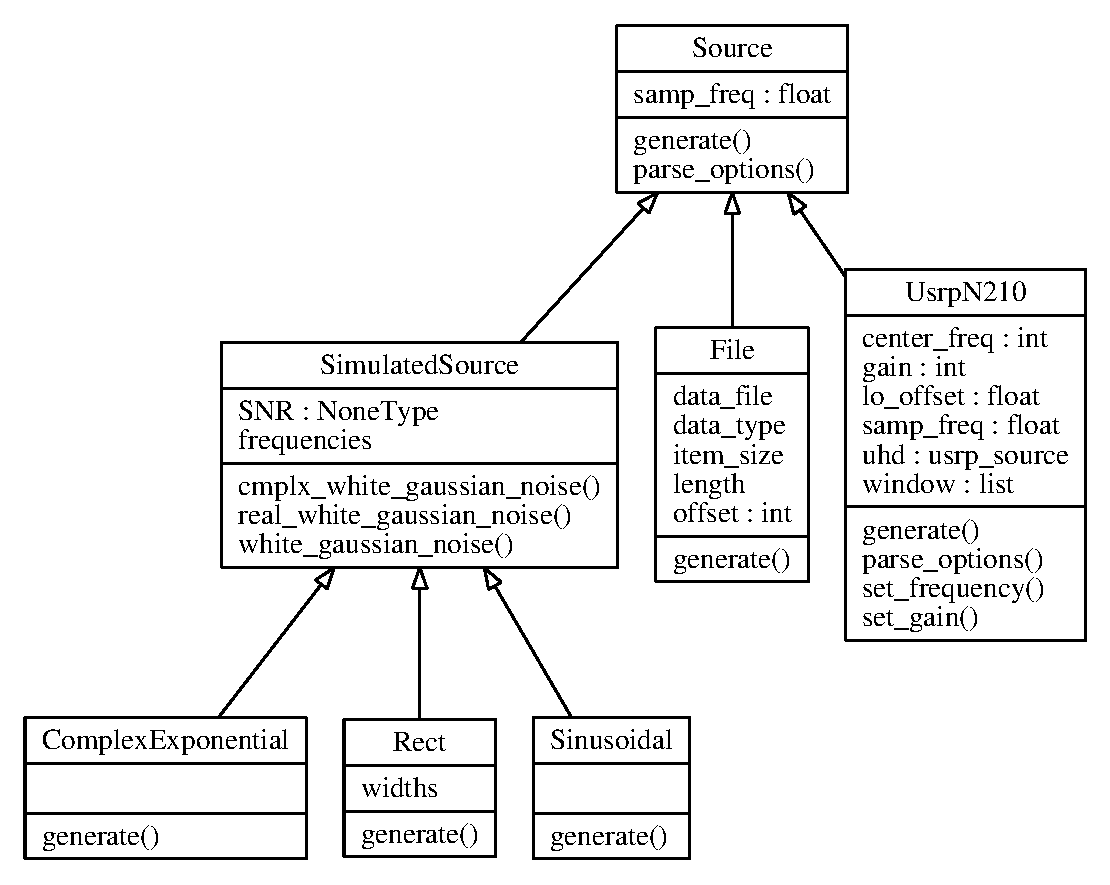
\includegraphics[width=\linewidth]{figures/classes_source.eps}
    \caption{The UML diagram of the sources}
    \label{fig:umlsource}
\end{figure}

\subsection{Simulated Source}
\label{sec:simulated-source}
The simulated sources are used for testing our algorithms. They generate samples on the fly, or use pre-recorded data. All the simulated sources have the same base class: \func{SimulatedSource}. This base class adds some utility methods to the sources to add Gaussian noise to the generated data.

\subsubsection{Sinusoidal}
The sinusoidal source generates a real valued signal, with a sum of sinusoidal signals with different frequencies. Because the signal is real valued this generates a symmetrical spectrum.

\subsubsection{Complex exponential}
The complex exponential source is the complex equivalent of the sinusoidal source. The generated complex signal is the sum of complex exponentials with different frequencies,

\subsubsection{Rectangular source}
The rectangular source generates a signal with multiple rectangles in the spectrum with specified frequencies and widths. The time domain signal is generated by adding multiple sinc functions.

\subsubsection{File source}
The file source reads the samples from a file. This was used to test with real world data, but still get reproducible results. The files can be generated with \lib{GNU Radio} using a file sink.


\subsection{USRP source}
For the USRPs we have two sources. One for normal operation for simulating different sampling methods. The other is for doing hardware co-prime sampling. The USRP sources also have methods to change the centre frequency and the gain of the front-end of the radio.

\subsubsection{Normal source}
The normal source uses the \func{finite\_acquisition} function. This provides a very easy way to get a specified number of samples from one USRP\@. This method has a few drawbacks (see \cref{sec:drivers}). The problems with the dc compensation of the local oscillator are prevented by shifting the local oscillator out of the sampled spectrum. Unfortunately this halves our effective bandwidth.

\subsubsection{Coprime source}
The coprime source uses an external \CC~program to do the actual sampling. This program synchronises the two streams and can sample from two USRPs with different sample rates. The samples are then sent over a socket to the coprime source in Python for further processing.


\section{Sampling}
\label{sec:sampling}
After the samples are generated, different sampling methods have to be applied. Each sampler implements an interface called \func{Sampler}. This interface implements two methods, a \func{sample(signal)} method to act on the input samples, and a \func{get\_C()} function that returns the sampling matrix\footnote{This is required for the reconstructors as their algorithms require knowledge about the sample intervals} used by the sampler.

\begin{figure}
    \centering
    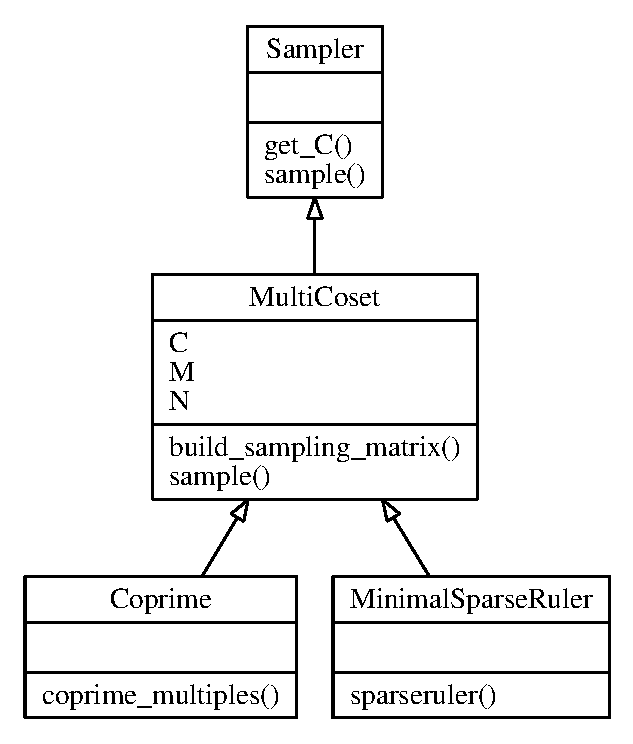
\includegraphics[width=0.5\linewidth]{./figures/classes_sampling.eps}
    \caption{The UML diagram of the samplers}
    \label{fig:}
\end{figure}

\subsection{Multi-coset sampler}
\label{sub:multi_coset_sampler}
Multi-coset sampling (as introduced in \cref{cha:sampling}) is based on a multiple device sampler. The crucial component here is the offset of the common sampling period (sometimes referred to as the `ruler' of a multi-coset system in context of the minimal sparse ruler problem). This sampler takes three arguments:
\begin{description}
    \item[S] is the list of offsets,
    \item[M] is the number of cosets, and
    \item[N] is the downsampling factor such that every coset samples the input signal once every N samples.
\end{description}
The list of offsets is used to generate the C matrix which has dimensions defined by M and N.

The method \func{sample(signal)} takes a signal, uniformly sampled, as argument and returns a multi-coset sampled signal. Our initial implementation used a loop and a matrix multiplication. To speed up this function the for loop was vectorized by a single matrix multiplication. This is achieved by reshaping the input signal to a matrix with one dimension N and the other determined by the length of the input signal.

\subsection{Minimal sparse ruler sampler}
\label{sec:multi-coset-sampler}
The minimal sparse ruler is a special case of the Multi-coset sampler. Its list offsets are all of a special form such that it forms a minimal sparse ruler on the downsampling factor. This means that implementation wise everything can be inherited from the multi-coset implementation except that it generates its own set of intervals from a lookup table containing precomputed solutions to the minimal sparse ruler problem. This sampler inherits the \func{sample(signal)} method from the multi-coset sampler.

\subsection{Coprime sampler}
\label{sec:coprime-sampler}
The coprime sampler is another special case of the multi-coset sampler. The only difference again is the way the list of offsets is generated. As explained in \cref{sec:coprime}, the coprime sampler rests on two samplers with different sampling ratios that have a coprime ratio. The constructor takes two arguments, a and b, the coprime ratios of the sample frequencies.

Coprime can be seen as a different form of multi-coset sampling, $a + b - 1$ are the number of cosets and $a \cdot b$ is the downsampling factor as can be read in \cref{sec:coprime}. This means that two samplers that have a coprime ratio have a shared period of $a \cdot b$.
In the implementation the coprime offsets are generated using a generator function\footnote{
    A generator function is a way to do `lazy' generation of values which translates to lower memory usage. In this case the gains are marginal but it is good form nonetheless.}
which keeps returning multiples of the coprime until their least common multiple, the downsampling ratio $a \cdot b$, is reached. This sampler also inherits the multi-coset \func{sample(signal)} method.

\subsection{Hardware coprime}
\label{sec:hardware-coprime}
The hardware coprime sampler does not get one vector with input samples, but two with a different number of samples from two samplers with different sample rates. The sampling matrix is constructed as with the normal coprime sampler. The two input vectors are then transformed in one output vector that matches the sampling matrix.

\section{Reconstruction}
\label{sec:reconstruction}
Two different kind of reconstruction methods are implemented. One similar to the one specified in \cite{ariananda2012compressive} the other is discussed in Part 1 of this thesis. Both reconstructors implement the interface \func{reconstructor} which has a contract for one method named \func{reconstruct(signal)}, see the UML in \cref{fig:umlreconstructor}. Both classes make use of the shared function \func{calc\_pseudoinverse(R)}. This is a wrapper around \lib{SciPy's} \func{pinv}, which calculates the pseudoinverse. Because this operation is quite time consuming for larger systems a caching mechanism was introduced to lower startup times.% It writes a file with the specific parameters (L and all the intervals) in the name away to a cache directory.

\subsection{CrossCorrelation}
\label{sub:crosscorrelation}
The \func{CrossCorrelation} class implementation is based on \cite{ariananda2012compressive}. The constructor takes 3 arguments (one optional):
\begin{description}
    \item[L] determines the maximum lag estimated of cross-correlation of the cosets,
    \item[C] is the sampling matrix used by one of the samplers. This is required for the reconstruction algorithm, and
    \item[cache] (default is True) is a boolean value that determines whether the pseudo-inverse can be loaded and saved to the cache. This is mainly used for test and profiling purposes.
\end{description}
The constructor gets the number of cosets and the down-sampling factor from the C matrix. It constructs an R matrix using the \func{cross\_correlation\_filters()} which takes the \func{block\_toeplitz(Rc0, Rc1)} helper function to build the R matrix from the filter correlations.

The \func{reconstruct(signal)} takes the pseudo-inverse and multiplies it with signal cross correlations, to reconstruct the autocorrelation of the original signal.

\subsection{Wessel}
\label{sub:wessel}
Wessel's reconstructor is a variation on the reconstruction technique implemented by \func{CrossCorrelation}. The theory is thoroughly described in the first part of this thesis. The constructor takes 3 arguments (one optional):
\begin{description}
    \item[L] determines the maximum lag estimated of cross-correlation of the cosets.
    \item[C] is the sampling matrix used by one of the samplers. This is required for the reconstruction algorithm.
    \item[cache] (default is True) is a boolean value that determines whether the pseudo-inverse can be loaded and saved to the cache. Mainly used for test and profiling purposes.
\end{description}
The constructor gets the number of cosets and the down-sampling factor from the C matrix. It constructs the R matrix in \func{constructR()}, which makes use of the \func{build\_D()}, \func{filter\_cross\_correlations()} and \func{build\_rcc()} as helper functions. These all build matrices as described in \cref{cha:reconstruction}. The difference between the \func{CrossCorrelation} reconstructor and this one are that the form of the pseudoinverse is more optimized for \lib{NumPy} in \func{Wessel}'s case. This is because of how the input signal should be structured. Because \lib{NumPy's} native way of saving matrices is in row-major order\footnote{This is the standard way of saving a array in C, two notable exceptions are \matlab and Fortran. Column major order is often called Fortran style.}.

The \func{reconstruct(signal)} takes the pseudo-inverse and multiplies it with output of \func{cross\_correlation\_signals(signal)} reshaped to a vector.

\begin{figure}
    \centering
    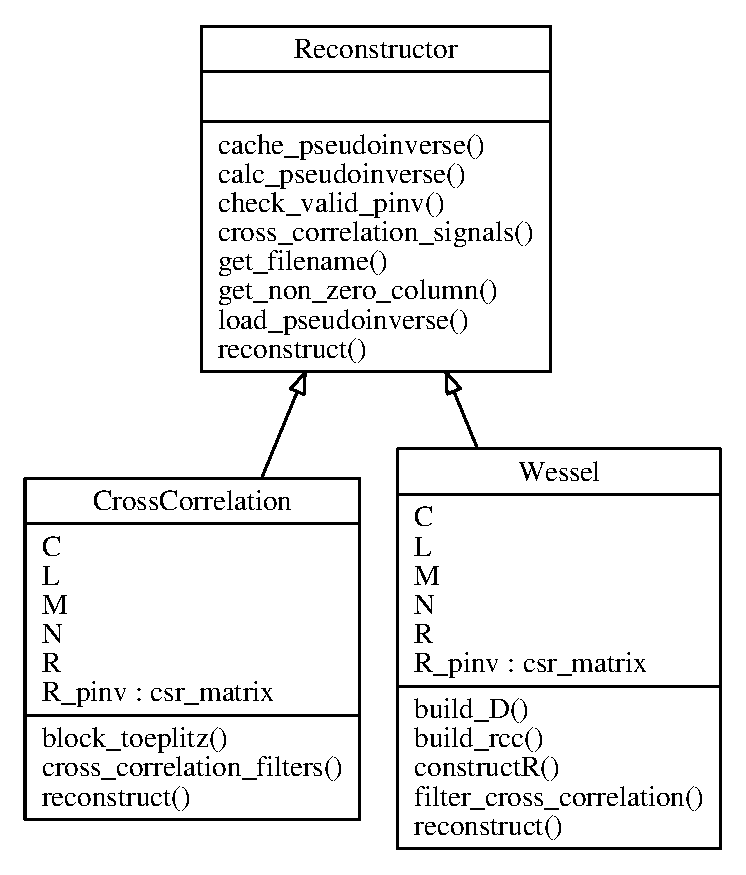
\includegraphics{./figures/classes_reconstruction.eps}
    \caption{The UML diagram of the reconstructors}
    \label{fig:umlreconstructor}
\end{figure}

\section{Detection}
\label{sec:detection}

\begin{figure}
    \centering
    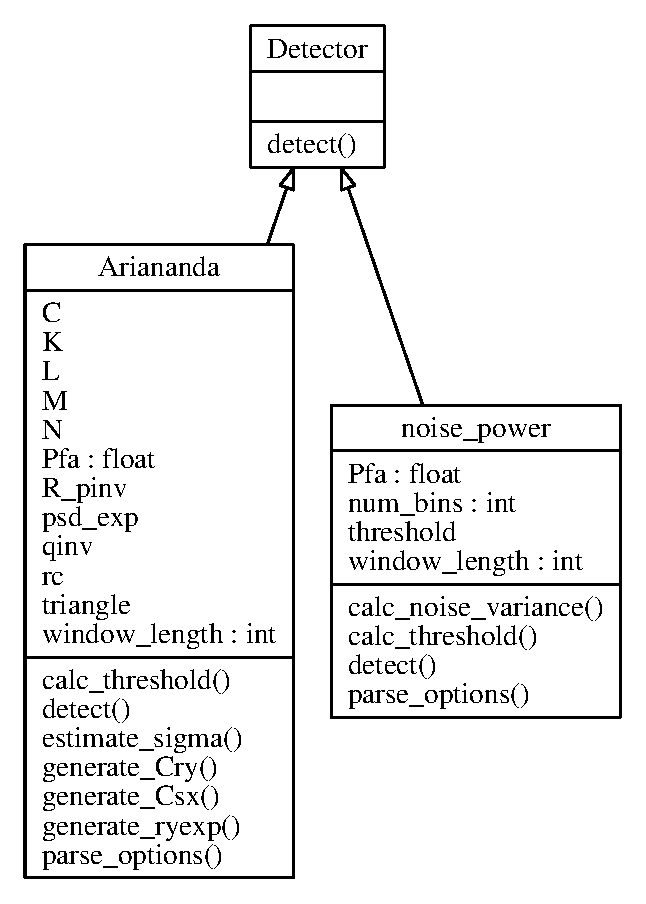
\includegraphics{./figures/classes_detection.eps}
    \caption{The UML diagram of the detectors}
    \label{fig:umldetector}
\end{figure}

\section{Utilities}
\label{sec:utilities}


\end{document}
